%% Creator: Inkscape inkscape 0.48.2, www.inkscape.org
%% PDF/EPS/PS + LaTeX output extension by Johan Engelen, 2010
%% Accompanies image file 'ASU_text.eps' (pdf, eps, ps)
%%
%% To include the image in your LaTeX document, write
%%   \input{<filename>.pdf_tex}
%%  instead of
%%   \includegraphics{<filename>.pdf}
%% To scale the image, write
%%   \def\svgwidth{<desired width>}
%%   \input{<filename>.pdf_tex}
%%  instead of
%%   \includegraphics[width=<desired width>]{<filename>.pdf}
%%
%% Images with a different path to the parent latex file can
%% be accessed with the `import' package (which may need to be
%% installed) using
%%   \usepackage{import}
%% in the preamble, and then including the image with
%%   \import{<path to file>}{<filename>.pdf_tex}
%% Alternatively, one can specify
%%   \graphicspath{{<path to file>/}}
%% 
%% For more information, please see info/svg-inkscape on CTAN:
%%   http://tug.ctan.org/tex-archive/info/svg-inkscape
%%
\begingroup%
  \makeatletter%
  \providecommand\color[2][]{%
    \errmessage{(Inkscape) Color is used for the text in Inkscape, but the package 'color.sty' is not loaded}%
    \renewcommand\color[2][]{}%
  }%
  \providecommand\transparent[1]{%
    \errmessage{(Inkscape) Transparency is used (non-zero) for the text in Inkscape, but the package 'transparent.sty' is not loaded}%
    \renewcommand\transparent[1]{}%
  }%
  \providecommand\rotatebox[2]{#2}%
  \ifx\svgwidth\undefined%
    \setlength{\unitlength}{480.89958443bp}%
    \ifx\svgscale\undefined%
      \relax%
    \else%
      \setlength{\unitlength}{\unitlength * \real{\svgscale}}%
    \fi%
  \else%
    \setlength{\unitlength}{\svgwidth}%
  \fi%
  \global\let\svgwidth\undefined%
  \global\let\svgscale\undefined%
  \makeatother%
  \begin{picture}(1,0.69511554)%
    \scriptsize		
    \put(0,0){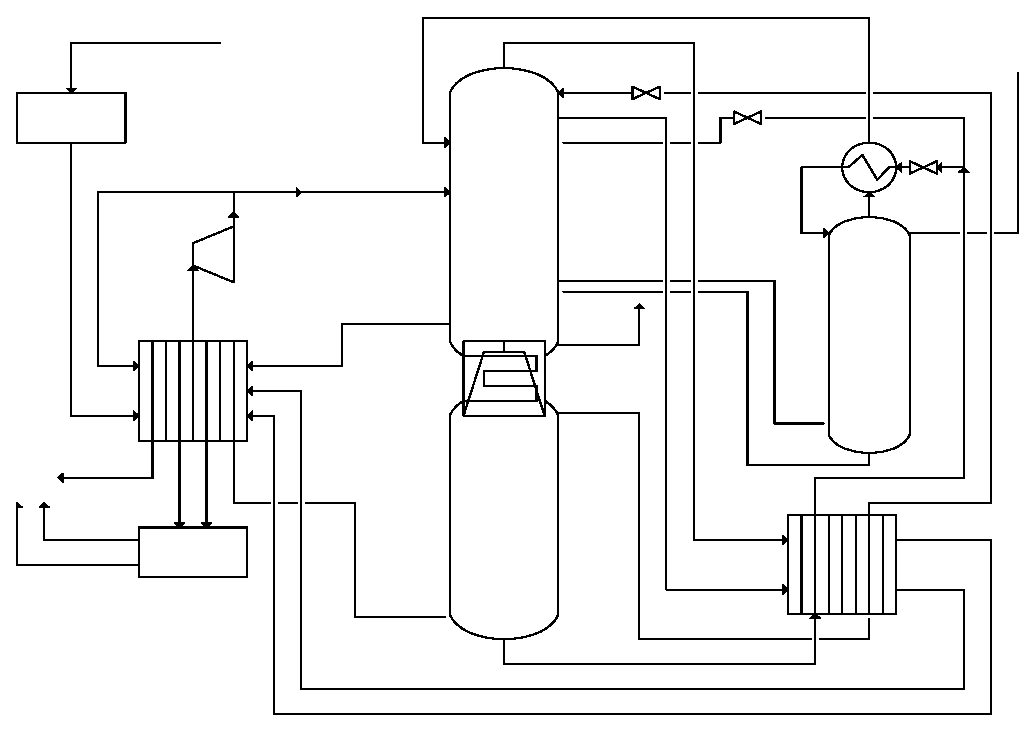
\includegraphics[width=\unitlength]{Pictures/ASU_text.eps}}%
    \put(0.47303574,0.48730942){\color[rgb]{0,0,0}\makebox(0,0)[lb]{\smash{LPC}}}%
    \put(0.4694296,0.20132682){\color[rgb]{0,0,0}\makebox(0,0)[lb]{\smash{HPC}}}%
    \put(0.83500402,0.38163476){\color[rgb]{0,0,0}\makebox(0,0)[lb]{\smash{CAC}}}%
    \put(0.05258426,0.59980743){\color[rgb]{0,0,0}\CM{compression \& \\ pre-purification}}%
    \put(0.14352294,0.15715136){\color[rgb]{0,0,0}\makebox(0,0)[lb]{\smash{liquefier}}}%
    \put(0.29858781,0.52588116){\color[rgb]{0,0,0}\makebox(0,0)[lb]{\smash{expanded air}}}%
    \put(0.38899094,0.33926244){\color[rgb]{0,0,0}\CM{condenser / \\�re-boiler}}%
    \put(0.32743709,0.39696094){\color[rgb]{0,0,0}\makebox(0,0)[lb]{\smash{gas oxygen}}}%
    \put(0.54290509,0.35549012){\color[rgb]{0,0,0}\makebox(0,0)[lb]{\smash{liquid oxygen}}}%
    \put(0.5699513,0.05437579){\color[rgb]{0,0,0}\makebox(0,0)[lb]{\smash{oxygen-rich liquid}}}%
    \put(0.59339131,0.00479107){\color[rgb]{0,0,0}\makebox(0,0)[lb]{\smash{gas nitrogen}}}%
    \put(0.99337587,0.51282048){\color[rgb]{0,0,0}\rotatebox{90}{\makebox(0,0)[lb]{\smash{crude argon}}}}%
    \put(0.58437597,0.03003421){\color[rgb]{0,0,0}\makebox(0,0)[lb]{\smash{waste nitrogen}}}%
    \put(0.54921586,0.43572716){\color[rgb]{0,0,0}\makebox(0,0)[lb]{\smash{argon feed}}}%
    \put(0.74214534,0.25361611){\color[rgb]{0,0,0}\makebox(0,0)[lb]{\smash{argon return}}}%
    \put(0.10115056,0.6764383){\color[rgb]{0,0,0}\makebox(0,0)[lb]{\smash{plant air}}}%
    \put(0.3598925,0.10215738){\color[rgb]{0,0,0}\makebox(0,0)[lb]{\smash{air feed}}}%
    \put(0.53298812,0.67373368){\color[rgb]{0,0,0}\makebox(0,0)[lb]{\smash{gas nitrogen}}}%
    \put(0.54560966,0.60070896){\color[rgb]{0,0,0}\makebox(0,0)[lb]{\smash{waste nitrogen}}}%
    \put(0.12754442,0.3960594){\color[rgb]{0,0,0}\CM{heat \\ exchanger}}%
    \put(0.75059149,0.21935756){\color[rgb]{0,0,0}\CM{heat \\�exchanger}}%
    \put(0.14262141,0.48170568){\color[rgb]{0,0,0}\makebox(0,0)[lb]{\smash{turbine}}}%
    \put(0.66010521,0.0805205){\color[rgb]{0,0,0}\makebox(0,0)[lb]{\smash{liquid nitrogen}}}%
  \end{picture}%
\endgroup%
